
%%%%%%%%%%%%%%
%%% DESIGN %%%
%%%%%%%%%%%%%%

Application Design
= how did we design the application

Design principles, inspiration, methodology

Design concerns for tabletops

scenarios

ranking of features

set of basic application commands
set of interaction strategies

preliminary usability study:
method
result analysis

Design choices

concept of META manipulation

\chapter{Preliminary user study}

Designing a software application is no easy task, and implies making crucial decisions.
AppName offers an unprecedented service and introduces new types of interaction, and thus challenging design.

A well-designed product is a successful one.
Usability and appeal are key elements towards the success of an application.
The goal of this experiment is to gather knowledge directly from users to inform important design decisions.

\section{Method}

Six interaction primitives were identified.
They refer to the most basic user interactions that the application should support.
\begin{enumerate}
\item{\emph{Dragging} the application window across the interactive surface.}
\item{\emph{Rotating} the application window across the interactive surface.}
\item{\emph{Resizing} the application window across the interactive surface.}
\item{\emph{Minimizing} the application window, making it possible to restore it easily.}
\item{\emph{Hiding} the content of the application window.}
\item{\emph{Exiting} the application, thus closing the application window.}
\end{enumerate}

Specific interaction strategies emerged from researching the different possibilities to implement those basic interactions.
Each strategy can be consistently implemented for all previously defined primitives.
\begin{enumerate}
\item{\emph{Action Tabs} are traditional buttons/tabs that implement functionalities.}
\item{The \emph{Action Bar} can be compared to a virtual touchpad, it includes a manipulation area and buttons.}
\item{\emph{Window Toggle} refers to using a switch to toggle the window between inactive and active states. In its inactive state, the window is made manipulable as a common digital picture.}
\item{The \emph{Active Border} is a digital frame around the application window used for manipulation.}
\item{\emph{Active Corners} is a strategy similar to Active Border, with the difference that the border's corners implement specific functionalities.}
\item{\emph{Other} regroups suggestions that do not fit with any specific strategy.}
\end{enumerate}


\begin{figure}[]
  \caption{Interaction primitives.}
  \centering
    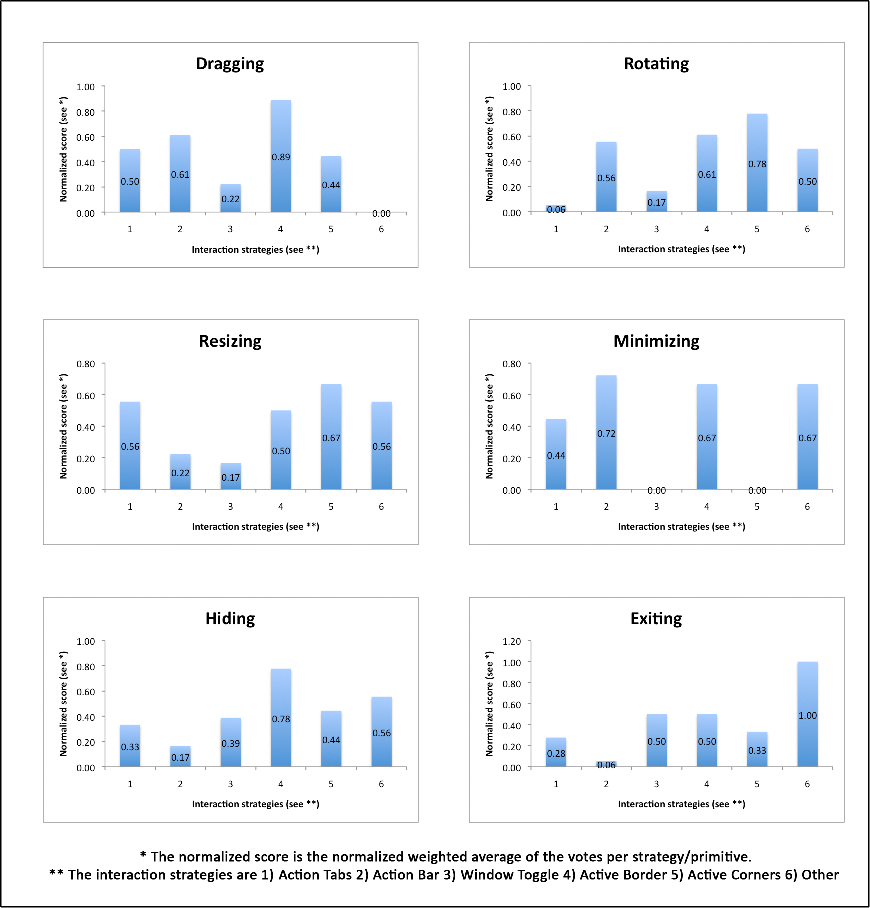
\includegraphics[]{images/primHistog}
\end{figure}

\begin{figure}[]
  \caption{Interaction strategies.}
  \centering
    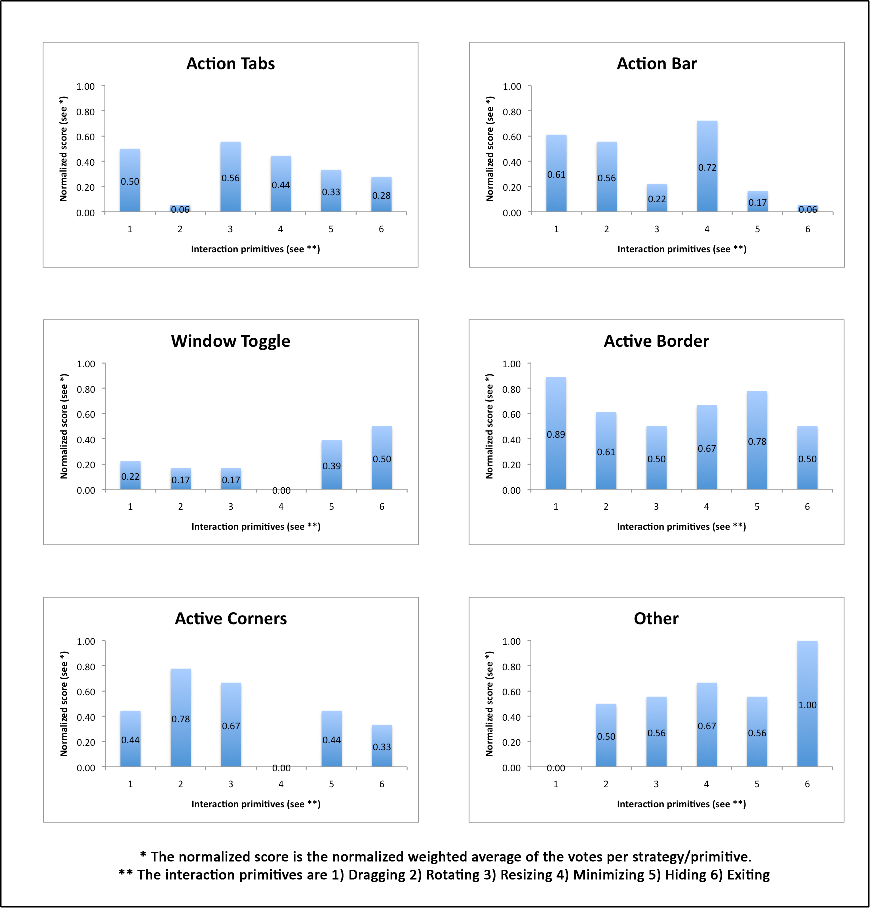
\includegraphics[]{images/stratHistog}
\end{figure}

